\chapter{Introduction}
\lhead{\thechapter \space Introduction}
\label{ch:introduction}
This introductory chapter provides the reader with background and contextual information regarding this project.

\section{Background Information}
\label{sec:background}
This report is a mandatory deliverable for the \gls{STG2} module offered by \gls{FHTenL}, with the deadline being on the 13th of January 2020. It is the final deliverable in combination with the final presentation, and indicates the end of the graduation internship. The report exists to document the assignment, the final status of the project for the time scope of the graduation internship, as well as the process and research done as a form of substantiation.

\section{Company Description}
Seacon's mission is to be the logistics chain director, with a focus on overseas logistics, forwarding and distribution and supply chain solutions. Warehousing forms a basis that is linked to the other core services. Since its foundation in 1985, Seacon has grown to boast more than 700 employees, at various strategic locations throughout Europe.

\section{Problem Description}
Seacon owns more than 235000 m\textsuperscript{2} of warehouse capacity, distributed across numerous locations. All these warehouses currently make use of employees that perform inventory control \& management tasks. Among these task are checking (specific) locations, counting the amount of items on a pallet, damage checking, and others. All this is currently done by sending employees to one or more locations to the aforementioned tasks manually. This kind of work is tedious and is generally not considered a desirable job by most, and thus employees are getting scarcer. An example of a warehouse layout can be found in figure \ref{fig:warehouse_layout}, where the rectangle boxes represent racks, and AA/AB/AC represent the unique IDs of each side of a rack.
\begin{figure}[h]
	\centering
	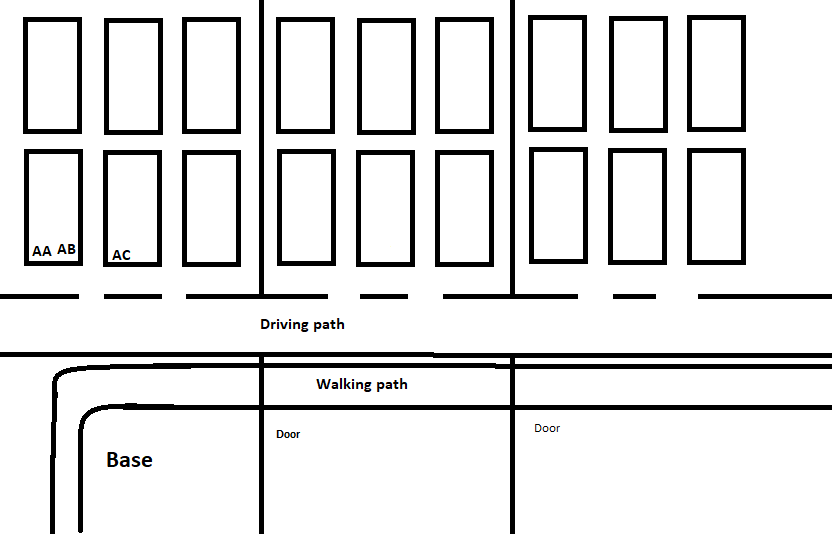
\includegraphics[width=0.75\linewidth]{img/sketch_warehouse_layout}
	\label{fig:warehouse_layout}
	\caption{Example layout of a warehouse.}
\end{figure}
\pagebreak

\section{Context}
\label{sec:context}
In order to combat employee scarceness, Seacon is looking to develop their own semi-autonomous solution for inventory and control management in their warehouses. All the tasks that the drones will eventually be responsible for are displayed in figure \ref{fig:roadmap}. Before all those tasks can be executed however, it is essential for the drone to fly a desired path without failure, which the collision avoidance solution will be used for.
\begin{figure}[h]
	\centering
	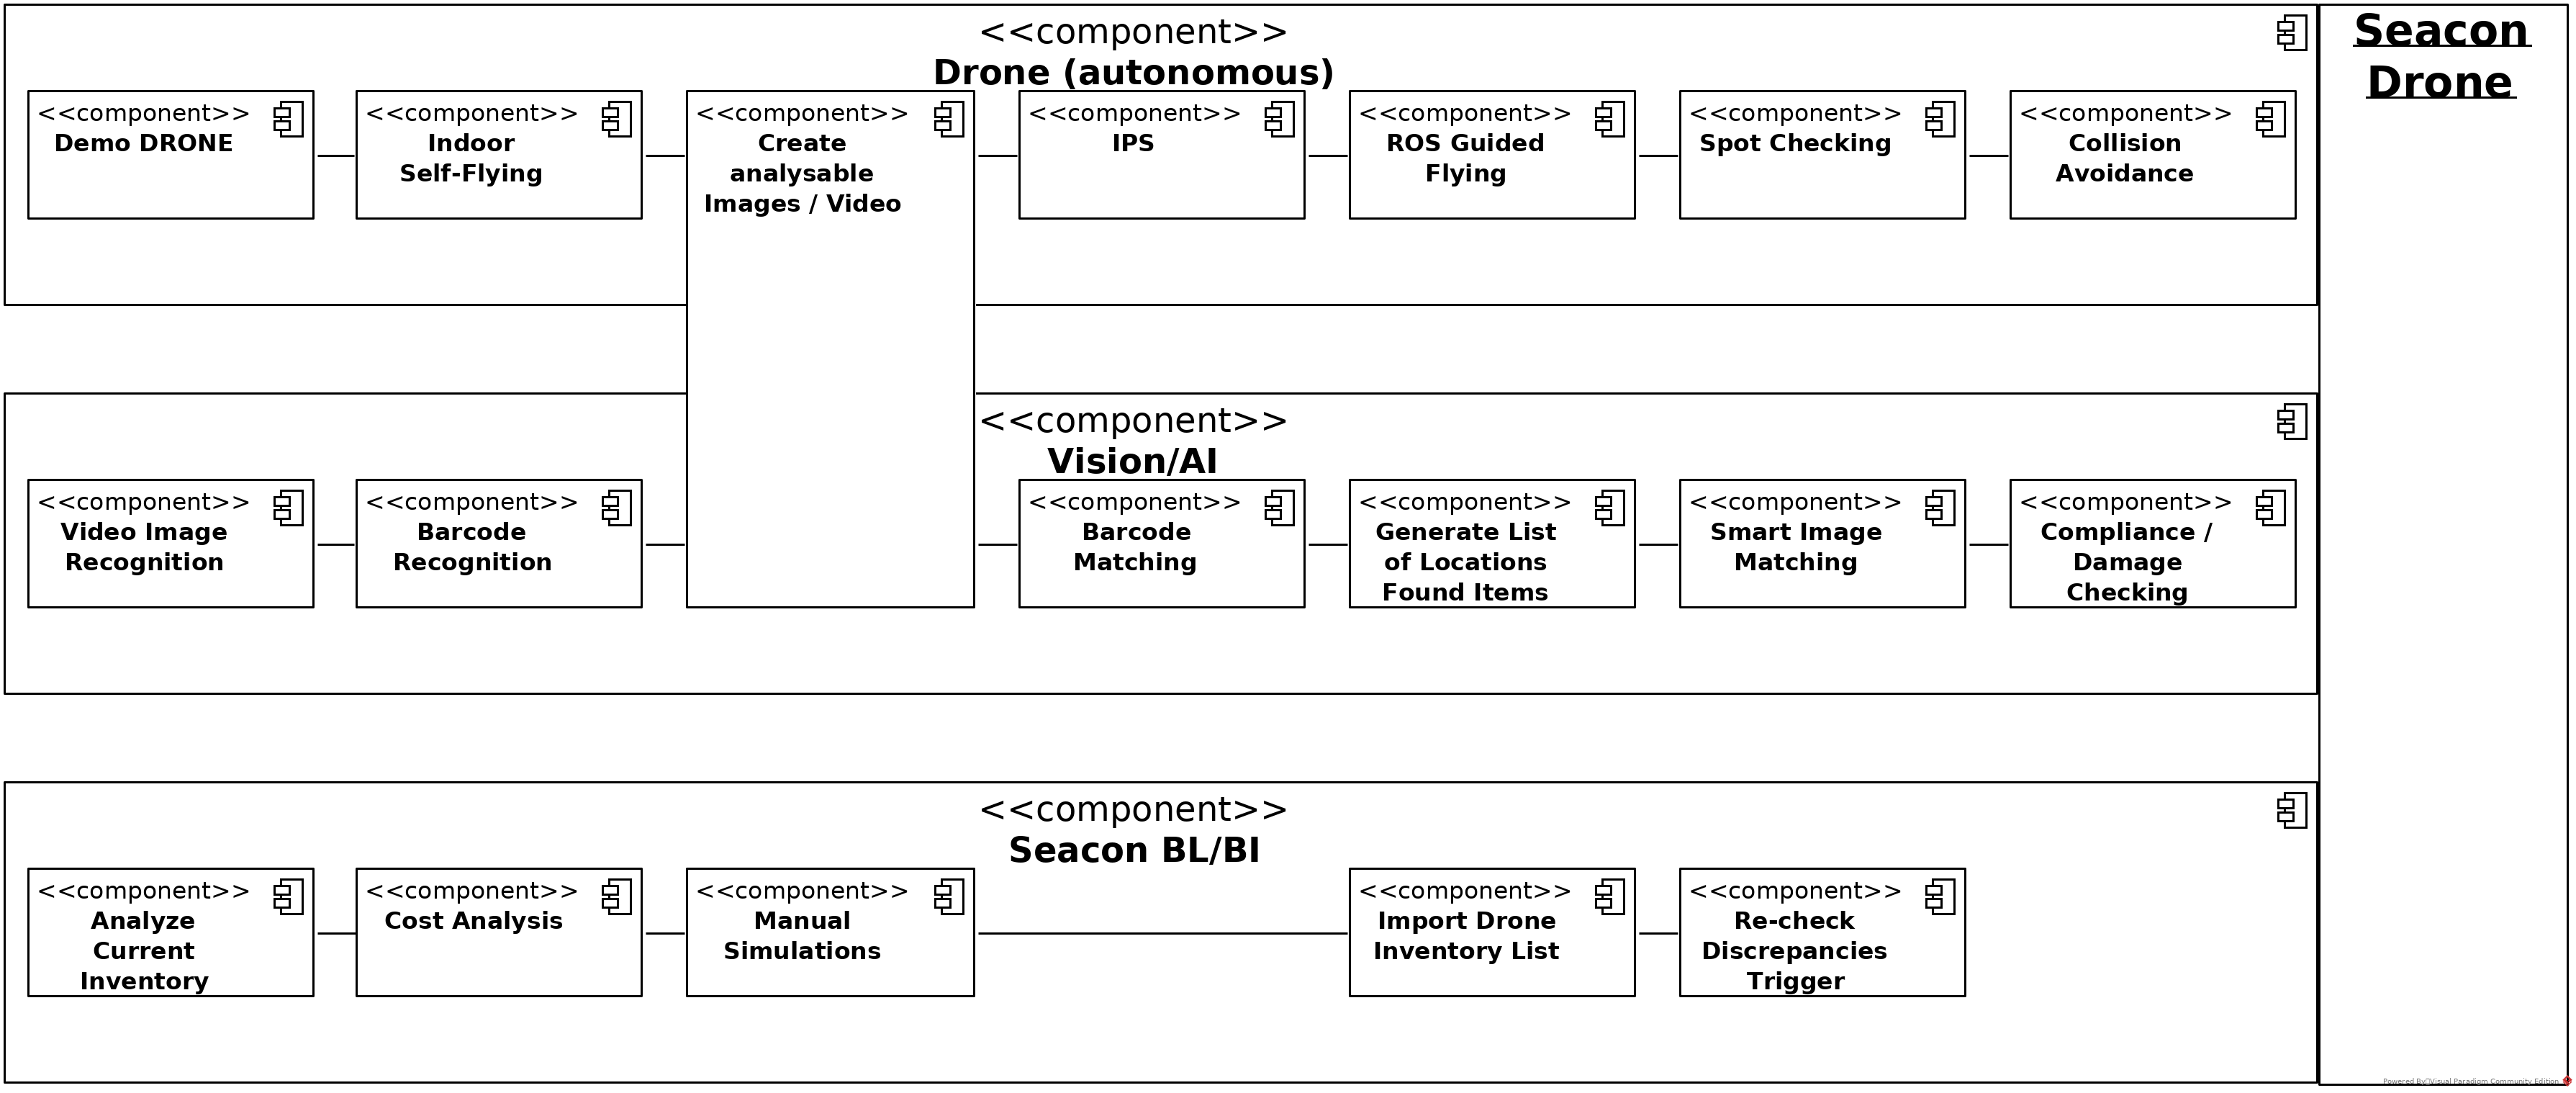
\includegraphics[width=\linewidth]{img/seacon_roadmap.png}
	\caption{Roadmap of the cycle count drone project.}
	\label{fig:roadmap}
\end{figure}

Due to the image size, the states the drone will traverse through can be found in appendix \ref{app:drone_states}. To display how tasks will eventually integrate, the scanning of bar-codes has also been added as an example task. At a later point in time, however, this could be replaced with a generic task state containing all the specific tasks as sub-states.

\section{Reporting Structure}
\label{sec:structure}
The remainder of this report will first cover a project description that lists stakeholders and defines the scope and risks. Secondly, possible approaches are described. Thirdly, the first developed concept using reinforcement learning is covered. This also includes information about the development of a simulation environment. Fourthly, the second developed concept using a state machine implementation is described. This chapter contains a requirements analysis, a state machine design, and information about the usage of computer vision for collision avoidance. Fifthly, a summary of the results is given and a conclusion is drawn from that. Finally, recommendations on how to proceed with this project are given.
